\chapter{Vorstudie}\label{Vorstudie}
%%%%%%%%%%%%%%%%%%%%%%%%%%%%%%%%%%%%%%%%%%%%%%%%%%%%%%%%%%%%%%%%%%%%%%%%%%%%%%%%
%Florian-Note:
%Hier würde ich dann als Überleitung erst mal drauf eingehen, wie die existierenden Arbeiten das Design der Vorstudie beeinflusst haben, also z.T. das, was Du jetzt grade in Kapitel 4 schreibst..
%%%%%%%%%%%%%%%%%%%%%%%%%%%%%%%%%%%%%%%%%%%%%%%%%%%%%%%%%%%%%%%%%%%%%%%%%%%%%%%%
%vorüberlegung mit - altes projekt aufsetzen, neues projekt machen?
%\todotext{Übergang - wie haben die Arbeiten das Design der Vorstudie beeinflusst?}\\
%\todotext{ist teilweise schon im kap.4}\\
%Anforderungsanalyse
Zu Beginn war es wichtig eine Anforderungsanalyse durchzuführen. Deshalb galt es, herauszufinden, in welchem Rahmen sich diese Arbeit bewegen sollte. Es bestanden die Optionen, ein fertiggestelltes Projekt anzupassen und zu verbessern oder ein vollkommen eigenes System zu entwickeln.
\\
Um zu erproben, wie ein bereits fertiges System funktioniert und wie es von Studenten und Mitarbeitern der Medienfakultät der BUW aufgenommen werden würde, habe ich die Entscheidung getroffen vorerst ein bereits vorhandenes Projekt herzunehmen und in der Praxis zu testen.
Da das Hermes System schon relativ alt war und hauptsächlich für PDA's entworfen wurde, kam es für den Test nicht in Frage.
Die Entscheidung fiel auf die zweite Version des NetBoards Projekts\cite{netboards:website} gewählt, da dieses Projekt zu dieser Zeit das aktuellste war.
\section{NetBoards Experiment}\label{NetBoards Experiment}
%\cite{apache:website}
%\cite{python:website}
Als Grundlage für meinen Experiment diente ein virtueller Debian-Linux Server mit 1,5GHz AMD CPU und 2GB RAM auf dem Apache2 als Webserver und Python2 für serverseitige Scripts liefen. Das öffentlich zugängliche NetBoards2 Projekt wurde installiert und konfiguriert.
\\
Nachdem der Server eingerichtet war kam die Frage auf, was als Anzeigegerät dienen sollte. Das originale Projekt von E. Wood wurde für 22 Zoll Monitore mit Touch-Oberfläche entworfen. Diese wurden vertikal neben die Büroeingänge gehangen.
\\
Da für mein Experiment nicht die notwendigen Ressourcen vorhanden waren, um den genauen Versuchsaufbau nachzuempfinden, fiel die Wahl des Anzeigegerätes auf einen kostengünstigen Tablet-PC.
\\
\todotext{was war das nochmal für ein tablet? 10Zoll? Spezifikationen angeben}
\\
Damit die Benutzer nicht mit den auf dem Gerät installierten Applikationen interagieren konnten wurde eine Kiosk-Applikation installiert.
Diese App schränkt die Interaktionsmöglichkeiten der Nutzer nur auf eine ausgewählte Webseite ein. Nur der Administrator des Gerätes hat die Möglichkeit diese zu ändern oder die Applikation ganz zu beenden.
\\
Ein weiteres Problem war die Befestigung des Displays.
Ich entschied mich dafür, das Tablet an den bereits vorhanden Türschildern anzubringen \abb{img:tuerschild}.
\begin{figure}[h!]
  \centering
    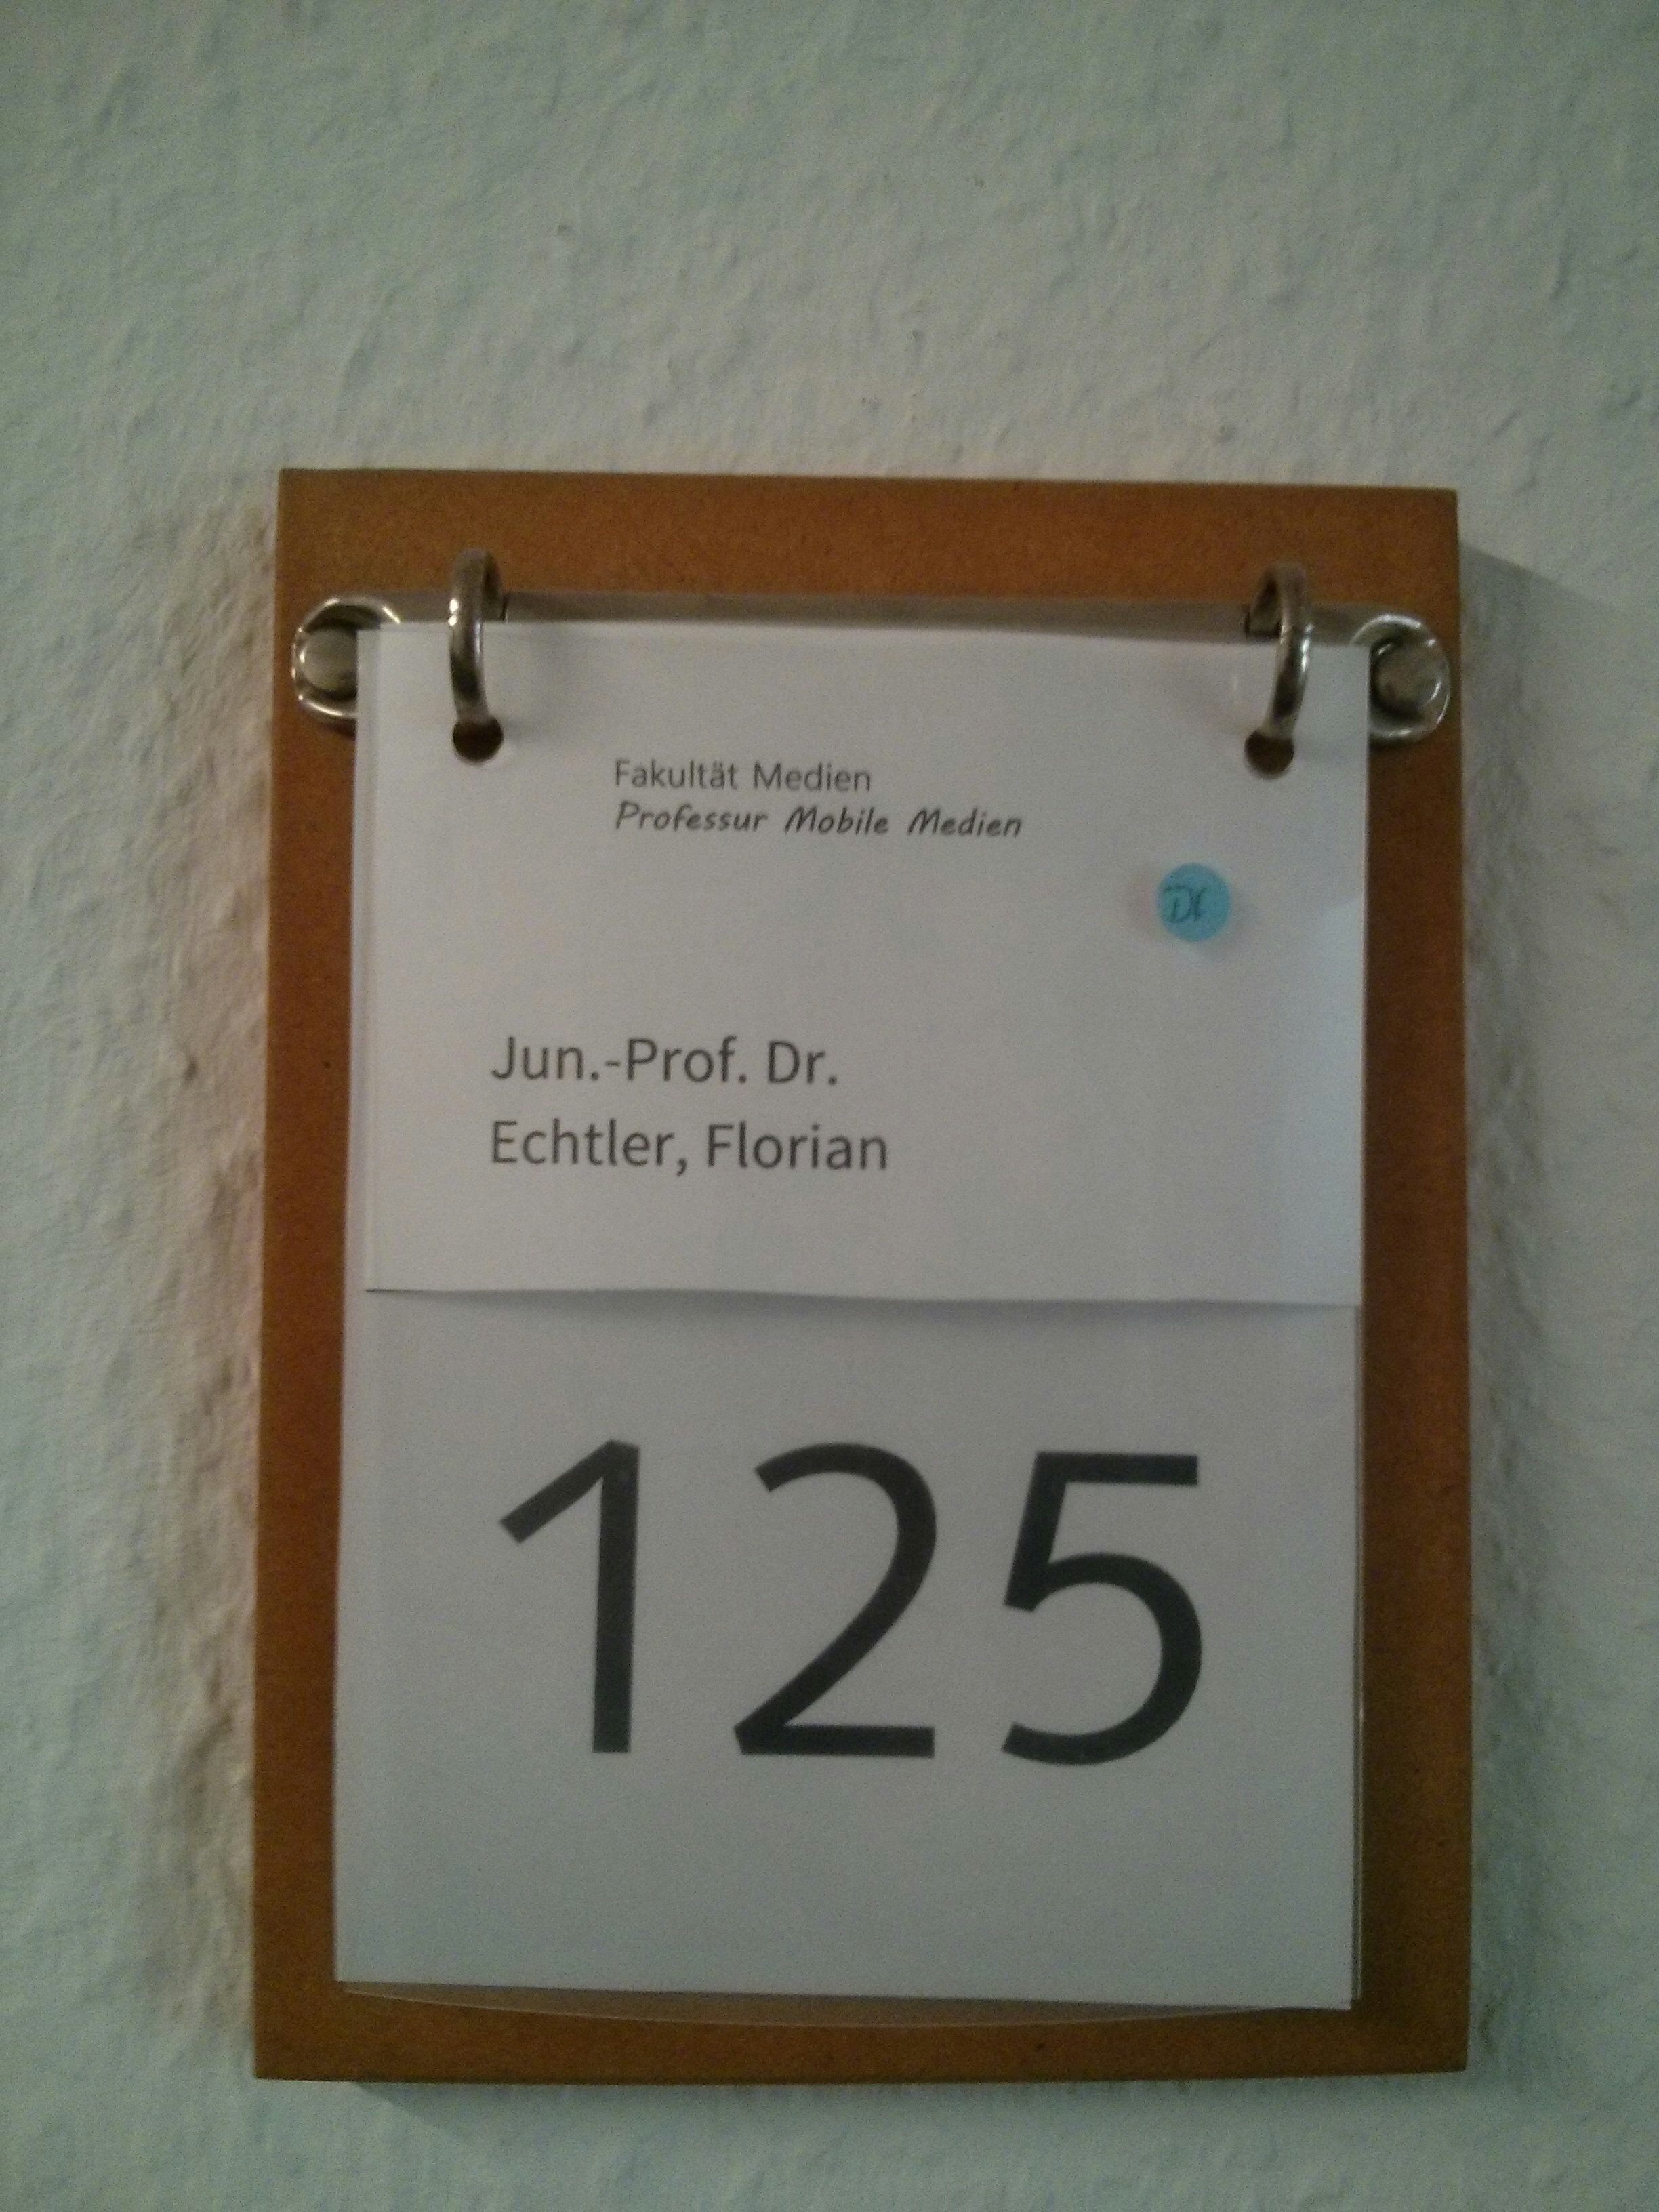
\includegraphics[width=0.5\textwidth]{./img/Tuerschild.jpg}
  \caption{Ein typisches Türschild in der Medienfakultät}
  \label{img:tuerschild}
\end{figure}\\
Dadurch, da sich die Rückwand des Tablets abschrauben ließ konnte ich zwei Löcher hinein bohren. Diese dienten zur Anbringung eines Drahtes, welcher über das Türschild gehangen werden konnte. Für dieses Experiment war die Aufhängung vollkommen ausreichend.
\\
Für die Stromversorgung wurde das Ladekabel des Tablets verlängert, damit es an eine Steckdose im Büro angeschlossen werden konnte.
\\
Als Testnutzer für das Experiment konnte ich zwei Mitarbeiter der Professur für Webtechnologien und Informationssysteme organisieren.
Diese Nutzer teilten sich ein Büro, wodurch nur ein Anzeigegerät benötigt wurde. Nach einer Einweisung zur Benutzung des Systems wurde klar, dass die zwei Tester nicht damit einverstanden waren, dass durch die Interaktivität des Boards jeder vorbeigehende Gast den dargestellten Inhalt nach belieben ändern konnte. Es hätte sein können, da durch die Anonymität der Gäste, das Board missbraucht werden könnte, um unangebrachte Skizzen zu zeichnen.
% Hier Beispiel mit Mensa Kinderhacksteak anstelle Rinderhacksteak
Aus diesem Grund habe ich für die Nutzer zwei verschiedene Ansichten erstellt:
\begin{itemize}
  \item Eine Backend-Sicht, auf der die Tester ihre Änderungen machen konnten.
  \item Eine Frontend-Sicht, die auf dem Tablet angezeigt wurde, nach 5 Minuten den aktuellen Stand abspeicherte und die Sicht auf den aktuellsten Stand der Backend-Sicht setzte.
\end{itemize}
\begin{figure}[h!]
  \centering
    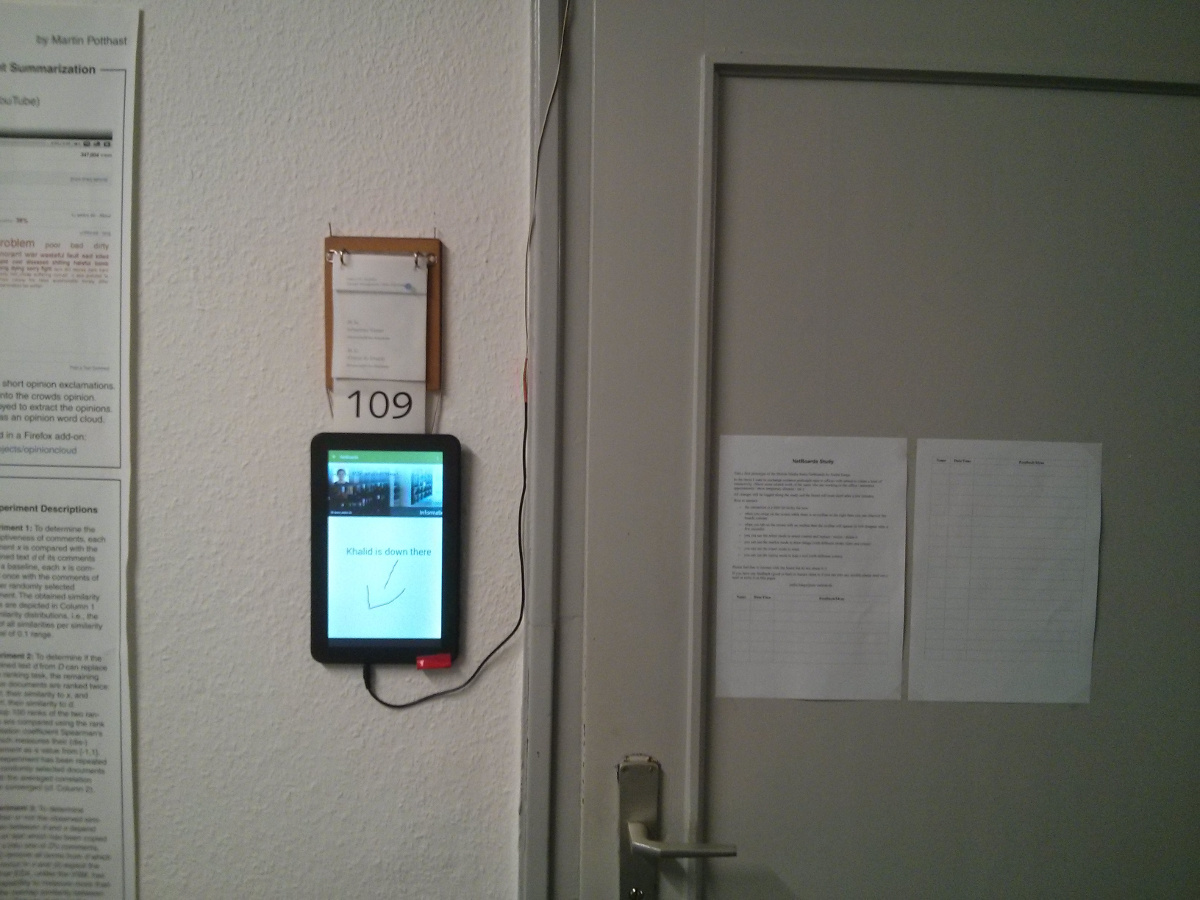
\includegraphics[width=0.7\textwidth]{./img/experiment01.jpg}
  \caption{Versuchsaufbau des Experiments}
  \label{img:experiment01}
\end{figure}



% Experiment Dauer
% 28.05.2015 - 08.06.2015
% 12 Tage
\section{Auswertung}\label{Auswertung}
Das Experiment lief 12 Tage. Die Nutzer erstellten sich zu Beginn einen Nutzeraccount und richteten ihr Board ein. Jeder der beiden lud ein Profilbild hoch und gab seinen Namen, sowie seinen akademischen Grad an.
Einer der Tester benutzte das Display um das Banner der Professur zu präsentieren \abb{img:experiment02} und um Gäste \bspw darüber zu informieren, dass er sich zur Zeit im Büro befindet \abb{img:experiment03}.
\\
Sehr erfreudig war, dass das Board viel Aufmerksamkeit zu erzeugen schien. Viele vorbeigehende Nutzer blieben stehen, um sich das Display genauer anzusehen und interagierten sogar damit. Dadurch entstanden viele Zeichnungen, wovon viele keinen tieferen Sinn hatten wie \bspw die Zeichnung in Abb. \ref{img:experiment04}. Jedoch gab es auch ab und an Nachrichten, die direkt an die Besitzer des Boards gerichtet waren, wie das Bild einer Kaffeetasse mit einem Fragezeichen aus Abb. \ref{img:experiment05}, was die Frage nach einer Kaffeepause darstellen sollte.
\begin{figure}[h!]
  \centering
    \subfigure[erste Änderung der Nutzer]{
      \frame{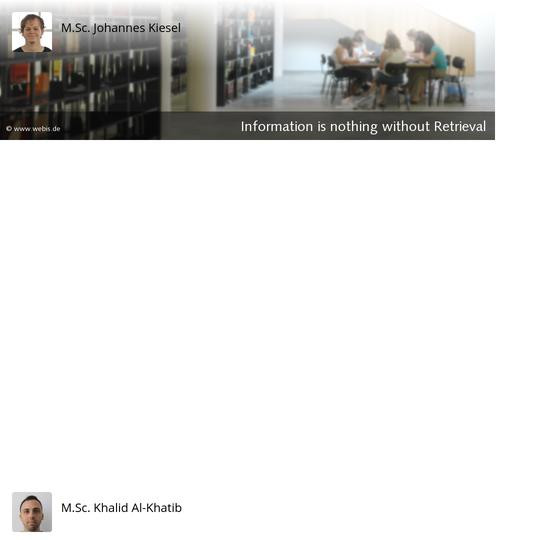
\includegraphics[width=0.4\textwidth]{./img/experiment02_empty.jpg}}
      \label{img:experiment02}
    }
    \subfigure[Statusangabe eines Nutzers]{
      \frame{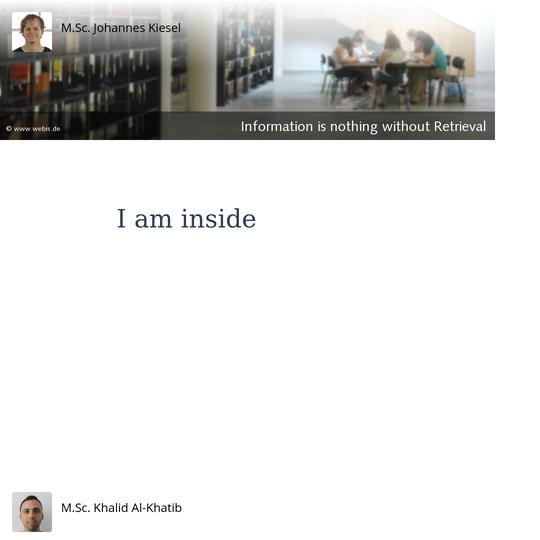
\includegraphics[width=0.4\textwidth]{./img/experiment03_statusContent.jpg}}
      \label{img:experiment03}
    }
    \subfigure[gezeichnetes Bild eines Gastes]{
      \frame{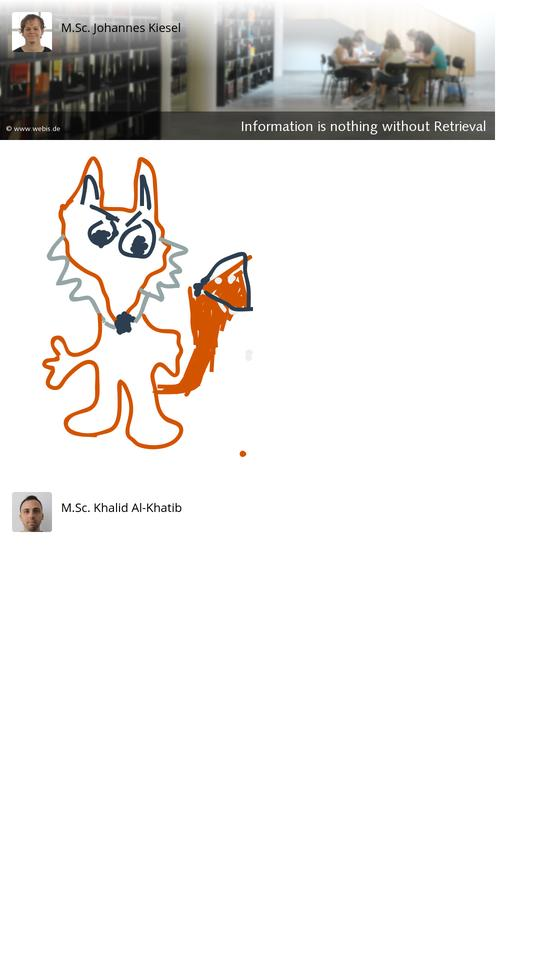
\includegraphics[width=0.4\textwidth]{./img/experiment04_fox.jpg}}
      \label{img:experiment04}
    }
    \subfigure[Frage eines Gastes]{
      \frame{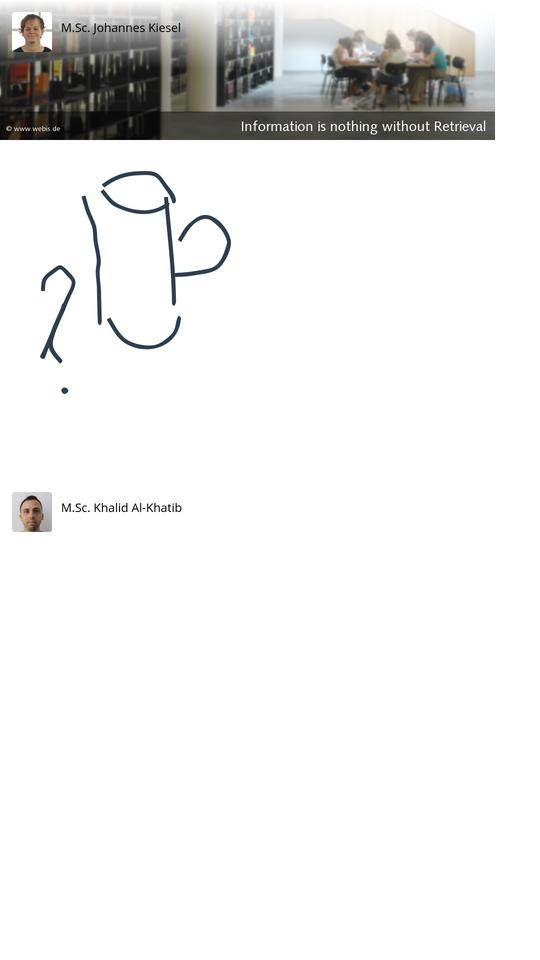
\includegraphics[width=0.4\textwidth]{./img/experiment05_coffee.jpg}}
      \label{img:experiment05}
    }
  \caption{Einige Beispielbilder}
\end{figure}
\\
\\
Nach Beendigung des Experiments führte ich ein Gespräch mit den Testnutzern, sowie mit einigen Gästen.
\\
Es stellte sich dabei heraus, dass durch die geringe Auflösung des Tablets den meisten Benutzern gar nicht klar wurde, dass zwei Nutzer auf dem Board angemeldet waren. Man musste manuell in der Ansicht scrollen, um den Inhalt des zweiten Nutzers einsehen zu können. Jedoch war auch das ein Problem, da Scrolling nur möglich war, wenn die Sidebar ausgeblendet war. Die meisten Nutzer interagierten demnach nur mit der oberen Hälfte des eigentlichen Inhalts.
\\
Ein weiteres Problem war, dass das Tablet eine sehr geringe Leistung hatte und das Touch-Interface nicht sehr genau war. Dadurch waren Interaktionen mit dem Board sehr langsam und ruckelig.
\\
Positive Äußerungen gab es bezüglich angezeigter Statusmeldungen wie \bspw ``I am inside''. Die meisten Besucher fanden diese Meldung hilfreich, da sie deshalb wussten, ob der Mitarbeiter zur Zeit im Raum ist.
Weil zum Empfangen einer Benachrichtigung eine Browser-App erforderlich war, was den Testern nicht bewusst war, hatten sie keine Möglichkeiten darüber benachrichtigt zu werden, wenn jemand etwas auf ihrem Board änderte. Es wäre besser gewesen, wenn die Besitzer einfach eine Email erhalten hätten, wenn ihnen jemand etwas mitteilen wollte.
\\
\\
Als Schlussfolgerung des Experimentes entschied ich mich dazu ein eigenes System zu entwerfen, da es mehr Sinn machte es von Grund auf nach den Anforderungen zu entwickeln, anstatt das NetBoards System so anzupassen, dass es die Anforderungen erfüllte.
Dieses sollte gut auf Tablets laufen und für eine kleinere Bildschirmgröße angepasst sein. Es erforderte, dass jeder Nutzer eine eigene Sicht bekommen sollte, da ansonsten auf dem Tablet zu wenig Platz wäre. Außerdem sollte es weniger als interaktives Whiteboard zu benutzen sein und mehr die Funktion von digitalen Pinnwänden übernehmen. Dadurch sollten nur noch die Besitzer die Möglichkeit haben den Angezeigten Inhalt zu ändern. Den Besuchern sollte dennoch möglich sein, mit den Besitzern in Kontakt zu treten, welche darauf eine Benachrichtiguns-Email erhalten sollten.